\documentclass[11pt,a4paper,notitlepage]{report}
% Shared preamble for the raw chapter-4 write-ups under docs/report/insights/.
%
% Each experiment_N/experiment_N.tex is a standalone, compilable LaTeX report
% written BEFORE anything goes into final_report/chapters/chapter_4_*.tex.
% It uses the final report's fonts, units and macros so that passages, tables
% and figures lift into the chapter without reformatting.
%
%   \documentclass[11pt,a4paper]{report}
%   % Shared preamble for the raw chapter-4 write-ups under docs/report/insights/.
%
% Each experiment_N/experiment_N.tex is a standalone, compilable LaTeX report
% written BEFORE anything goes into final_report/chapters/chapter_4_*.tex.
% It uses the final report's fonts, units and macros so that passages, tables
% and figures lift into the chapter without reformatting.
%
%   \documentclass[11pt,a4paper]{report}
%   % Shared preamble for the raw chapter-4 write-ups under docs/report/insights/.
%
% Each experiment_N/experiment_N.tex is a standalone, compilable LaTeX report
% written BEFORE anything goes into final_report/chapters/chapter_4_*.tex.
% It uses the final report's fonts, units and macros so that passages, tables
% and figures lift into the chapter without reformatting.
%
%   \documentclass[11pt,a4paper]{report}
%   \input{../common/preamble}
%   \begin{document} ...
%
% Figures and tables are NOT copied: \graphicspath and \reporttable resolve into
% final_report/figures/ and final_report/tables/, so the raw write-up always
% shows the same artefacts as the chapter.  Compile with:  latexmk -pdf <file>

\usepackage[T1]{fontenc}
\usepackage[utf8]{inputenc}
\usepackage{mathptmx}
\usepackage[scaled=0.92]{helvet}
\usepackage{courier}
\usepackage[a4paper,left=30mm,right=20mm,top=25mm,bottom=25mm]{geometry}
\usepackage{microtype}
\usepackage{booktabs}
\usepackage{tabularx}
\usepackage{longtable}
\usepackage{array}
\usepackage{multirow}
\usepackage{amsmath}
\usepackage{amssymb}
\usepackage{ifthen}
\usepackage{siunitx}
\usepackage{graphicx}
\usepackage{placeins}
\usepackage{caption}
\usepackage{enumitem}
\usepackage[table]{xcolor}
\usepackage{rotating}
\PassOptionsToPackage{hyphens}{url}\usepackage{url}
\usepackage[hidelinks]{hyperref}
\usepackage[nameinlink,noabbrev]{cleveref}

\graphicspath{{../../final_report/}{../../final_report/figures/}}
% \reporttable{name} inputs final_report/tables/name.tex
\newcommand{\reporttable}[1]{\input{../../final_report/tables/#1}}

\newcommand{\repo}[1]{\texttt{\detokenize{#1}}}
\sisetup{detect-all,group-separator={,},range-phrase=--,range-units=single}
\DeclareSIUnit{\pixel}{px}
\DeclareSIUnit{\mebi}{Mi}
\captionsetup{font=small,labelfont=bf}
\setlist{nosep}
\setlength{\parskip}{4pt}
\setlength{\LTcapwidth}{\textwidth}

% ---- result-slot status (RENDERED here, unlike in the final report)
\definecolor{stcompleted}{HTML}{A5D6A7}
\definecolor{stpartial}{HTML}{FFF2CC}
\definecolor{stuntested}{HTML}{FFD8A8}
\definecolor{stblocked}{HTML}{FFCDD2}
\definecolor{stfailed}{HTML}{FFCDD2}
\definecolor{stplanned}{HTML}{E0E0E0}
\newcommand{\slotstatus}[2]{%
  \par\noindent\fcolorbox{black!40}{st#1}{\parbox{\dimexpr\textwidth-2\fboxsep-2\fboxrule}{%
    \textbf{Status: #1.}\ #2}}\par\medskip}
\newcommand{\status}[1]{\textbf{#1}}

% ---- queries: RENDERED in red here so a reader sees every open concern in place
\definecolor{flagred}{HTML}{B00000}
\newcommand{\flag}[1]{\textcolor{flagred}{#1}}
\newcommand{\moved}[1]{#1}
\newenvironment{queried}[1][Questionable]%
  {\par\addvspace{0.6ex}\begingroup\color{flagred}\noindent
   \textbf{[#1]}\ \ignorespaces}%
  {\par\endgroup\addvspace{0.6ex}}

% ---- per-block performance marks (section 4.5 diagrams)
\definecolor{perfgood}{HTML}{A5D6A7}
\definecolor{perfpoor}{HTML}{FFCDD2}
\definecolor{perfnoeffect}{HTML}{D9EAF7}
\definecolor{perfnone}{HTML}{FFF2CC}
\newcommand{\perfmark}[1]{%
  \ifthenelse{\equal{#1}{good}}{\colorbox{perfgood}{\scriptsize good}}{%
  \ifthenelse{\equal{#1}{poor}}{\colorbox{perfpoor}{\scriptsize poor}}{%
  \ifthenelse{\equal{#1}{noeffect}}{\colorbox{perfnoeffect}{\scriptsize no effect}}{%
  \colorbox{perfnone}{\scriptsize no claim}}}}}

%   \begin{document} ...
%
% Figures and tables are NOT copied: \graphicspath and \reporttable resolve into
% final_report/figures/ and final_report/tables/, so the raw write-up always
% shows the same artefacts as the chapter.  Compile with:  latexmk -pdf <file>

\usepackage[T1]{fontenc}
\usepackage[utf8]{inputenc}
\usepackage{mathptmx}
\usepackage[scaled=0.92]{helvet}
\usepackage{courier}
\usepackage[a4paper,left=30mm,right=20mm,top=25mm,bottom=25mm]{geometry}
\usepackage{microtype}
\usepackage{booktabs}
\usepackage{tabularx}
\usepackage{longtable}
\usepackage{array}
\usepackage{multirow}
\usepackage{amsmath}
\usepackage{amssymb}
\usepackage{ifthen}
\usepackage{siunitx}
\usepackage{graphicx}
\usepackage{placeins}
\usepackage{caption}
\usepackage{enumitem}
\usepackage[table]{xcolor}
\usepackage{rotating}
\PassOptionsToPackage{hyphens}{url}\usepackage{url}
\usepackage[hidelinks]{hyperref}
\usepackage[nameinlink,noabbrev]{cleveref}

\graphicspath{{../../final_report/}{../../final_report/figures/}}
% \reporttable{name} inputs final_report/tables/name.tex
\newcommand{\reporttable}[1]{\input{../../final_report/tables/#1}}

\newcommand{\repo}[1]{\texttt{\detokenize{#1}}}
\sisetup{detect-all,group-separator={,},range-phrase=--,range-units=single}
\DeclareSIUnit{\pixel}{px}
\DeclareSIUnit{\mebi}{Mi}
\captionsetup{font=small,labelfont=bf}
\setlist{nosep}
\setlength{\parskip}{4pt}
\setlength{\LTcapwidth}{\textwidth}

% ---- result-slot status (RENDERED here, unlike in the final report)
\definecolor{stcompleted}{HTML}{A5D6A7}
\definecolor{stpartial}{HTML}{FFF2CC}
\definecolor{stuntested}{HTML}{FFD8A8}
\definecolor{stblocked}{HTML}{FFCDD2}
\definecolor{stfailed}{HTML}{FFCDD2}
\definecolor{stplanned}{HTML}{E0E0E0}
\newcommand{\slotstatus}[2]{%
  \par\noindent\fcolorbox{black!40}{st#1}{\parbox{\dimexpr\textwidth-2\fboxsep-2\fboxrule}{%
    \textbf{Status: #1.}\ #2}}\par\medskip}
\newcommand{\status}[1]{\textbf{#1}}

% ---- queries: RENDERED in red here so a reader sees every open concern in place
\definecolor{flagred}{HTML}{B00000}
\newcommand{\flag}[1]{\textcolor{flagred}{#1}}
\newcommand{\moved}[1]{#1}
\newenvironment{queried}[1][Questionable]%
  {\par\addvspace{0.6ex}\begingroup\color{flagred}\noindent
   \textbf{[#1]}\ \ignorespaces}%
  {\par\endgroup\addvspace{0.6ex}}

% ---- per-block performance marks (section 4.5 diagrams)
\definecolor{perfgood}{HTML}{A5D6A7}
\definecolor{perfpoor}{HTML}{FFCDD2}
\definecolor{perfnoeffect}{HTML}{D9EAF7}
\definecolor{perfnone}{HTML}{FFF2CC}
\newcommand{\perfmark}[1]{%
  \ifthenelse{\equal{#1}{good}}{\colorbox{perfgood}{\scriptsize good}}{%
  \ifthenelse{\equal{#1}{poor}}{\colorbox{perfpoor}{\scriptsize poor}}{%
  \ifthenelse{\equal{#1}{noeffect}}{\colorbox{perfnoeffect}{\scriptsize no effect}}{%
  \colorbox{perfnone}{\scriptsize no claim}}}}}

%   \begin{document} ...
%
% Figures and tables are NOT copied: \graphicspath and \reporttable resolve into
% final_report/figures/ and final_report/tables/, so the raw write-up always
% shows the same artefacts as the chapter.  Compile with:  latexmk -pdf <file>

\usepackage[T1]{fontenc}
\usepackage[utf8]{inputenc}
\usepackage{mathptmx}
\usepackage[scaled=0.92]{helvet}
\usepackage{courier}
\usepackage[a4paper,left=30mm,right=20mm,top=25mm,bottom=25mm]{geometry}
\usepackage{microtype}
\usepackage{booktabs}
\usepackage{tabularx}
\usepackage{longtable}
\usepackage{array}
\usepackage{multirow}
\usepackage{amsmath}
\usepackage{amssymb}
\usepackage{ifthen}
\usepackage{siunitx}
\usepackage{graphicx}
\usepackage{placeins}
\usepackage{caption}
\usepackage{enumitem}
\usepackage[table]{xcolor}
\usepackage{rotating}
\PassOptionsToPackage{hyphens}{url}\usepackage{url}
\usepackage[hidelinks]{hyperref}
\usepackage[nameinlink,noabbrev]{cleveref}

\graphicspath{{../../final_report/}{../../final_report/figures/}}
% \reporttable{name} inputs final_report/tables/name.tex
\newcommand{\reporttable}[1]{\input{../../final_report/tables/#1}}

\newcommand{\repo}[1]{\texttt{\detokenize{#1}}}
\sisetup{detect-all,group-separator={,},range-phrase=--,range-units=single}
\DeclareSIUnit{\pixel}{px}
\DeclareSIUnit{\mebi}{Mi}
\captionsetup{font=small,labelfont=bf}
\setlist{nosep}
\setlength{\parskip}{4pt}
\setlength{\LTcapwidth}{\textwidth}

% ---- result-slot status (RENDERED here, unlike in the final report)
\definecolor{stcompleted}{HTML}{A5D6A7}
\definecolor{stpartial}{HTML}{FFF2CC}
\definecolor{stuntested}{HTML}{FFD8A8}
\definecolor{stblocked}{HTML}{FFCDD2}
\definecolor{stfailed}{HTML}{FFCDD2}
\definecolor{stplanned}{HTML}{E0E0E0}
\newcommand{\slotstatus}[2]{%
  \par\noindent\fcolorbox{black!40}{st#1}{\parbox{\dimexpr\textwidth-2\fboxsep-2\fboxrule}{%
    \textbf{Status: #1.}\ #2}}\par\medskip}
\newcommand{\status}[1]{\textbf{#1}}

% ---- queries: RENDERED in red here so a reader sees every open concern in place
\definecolor{flagred}{HTML}{B00000}
\newcommand{\flag}[1]{\textcolor{flagred}{#1}}
\newcommand{\moved}[1]{#1}
\newenvironment{queried}[1][Questionable]%
  {\par\addvspace{0.6ex}\begingroup\color{flagred}\noindent
   \textbf{[#1]}\ \ignorespaces}%
  {\par\endgroup\addvspace{0.6ex}}

% ---- per-block performance marks (section 4.5 diagrams)
\definecolor{perfgood}{HTML}{A5D6A7}
\definecolor{perfpoor}{HTML}{FFCDD2}
\definecolor{perfnoeffect}{HTML}{D9EAF7}
\definecolor{perfnone}{HTML}{FFF2CC}
\newcommand{\perfmark}[1]{%
  \ifthenelse{\equal{#1}{good}}{\colorbox{perfgood}{\scriptsize good}}{%
  \ifthenelse{\equal{#1}{poor}}{\colorbox{perfpoor}{\scriptsize poor}}{%
  \ifthenelse{\equal{#1}{noeffect}}{\colorbox{perfnoeffect}{\scriptsize no effect}}{%
  \colorbox{perfnone}{\scriptsize no claim}}}}}

\setcounter{chapter}{4}
\renewcommand{\thesection}{4.2.\arabic{section}}
\renewcommand{\thefigure}{2.\arabic{figure}}
\renewcommand{\thetable}{2.\arabic{table}}
\title{Experiment 2: Offline YOLO Detector Performance\\
       \large Raw write-up for Chapter 4, Section 4.2}
\author{Bolton Athit Davies}
\date{Reporting cutoff: 22 October 2026}
\begin{document}
\maketitle

\noindent\textbf{Purpose of this document.} This is the raw, complete write-up
of Experiment~2, written before the thesis chapter; Section~4.2 of the final
report is extracted from it. Every number traces to a file under
\repo{output/} named in the ``Reporting rules'' paragraph of its slot.

% =====================================================================
\section{Simulation}
\label{sec:exp2-sim}

\slotstatus{completed}{Four dynamic recordings, \num{9860} left-camera frames,
scored against projected simulator ground truth at a single confidence
threshold.}

\paragraph{Objective.} Measure how well the project detector localises and
names warehouse objects, independently of either SLAM integration, so that the
dynamic filters of Experiment~3 have a known input quality.

\paragraph{Process.} The collision mesh of every prop was projected into
\repo{cam0} at each frame to form ground-truth boxes, the project checkpoint
\repo{weight/best.pt} was run on the same frames, and predictions were matched
to truth by IoU. Overlays from every recording were inspected before the
aggregates were accepted (\cref{fig:exp2-overlay}). Class assignment was then
scored separately, on the matched pairs only, so that a naming error is never
confused with a localisation error.

\paragraph{Datasets.} The four scripted dynamic recordings of the extreme
world (\cref{tab:exp2-datasets}). Every recording has the plain floor and 68
or 69 placed props, of which the moving ones follow scripted paths.

\begin{table}[htbp]
\centering
\caption{Recordings scored in Experiment~2 (names without the \repo{dataset_} prefix). Objects, route length and
simulated span are from the dataset registry; frames are the left-camera
images the detector was scored on.}
\label{tab:exp2-datasets}
\small
\begin{tabular}{llrrrr}
\toprule
Recording & Arrangement & Objects & Route [\si{\metre}] & Span [\si{\second}] & Frames \\
\midrule
\repo{dynamic_nofloortexture_00_000} & dynamic\_00 & 69 & 97.1 & 77.4 & \num{2347} \\
\repo{dynamic_nofloortexture_00_001} & dynamic\_00 & 69 & 97.3 & 74.2 & \num{2236} \\
\repo{dynamic_nofloortexture_01_000} & dynamic\_01 & 68 & 122.8 & 84.6 & \num{2564} \\
\repo{dynamic_nofloortexture_02_000} & dynamic\_02 & 68 & 126.6 & 89.5 & \num{2713} \\
\midrule
Pooled & & & & & \num{9860} \\
\bottomrule
\end{tabular}
\end{table}

\paragraph{Reporting rules.} Confidence threshold \num{0.35}, NMS IoU
\num{0.50}, matching IoU \num{0.50}; an object counts as moving above
\SI{0.05}{\metre\per\second} from its pose history. Three exemptions remove
objects from scoring: truth boxes under \SI{12}{px} on a side are dropped,
truth covered more than \SI{70}{\percent} by a nearer object is neither hit
nor miss, and a prediction more than half covered by unlabelled scenery is
neither credited nor penalised. Pooled scores are micro-averages of the TP,
FP and FN counts over all frames, not means of the four per-recording scores.
Class metrics are computed only on pairs associated at IoU $\ge 0.50$ without
requiring class agreement. Average precision is not reported because only
predictions above the single threshold were retained. Source: \path{script/yolo_eval.py}, which writes
\path{summary_metrics.csv}, \path{classification_metrics.csv} and the
per-recording overlay folders under \path{output/yolo_eval/}; the
exemption-matched recall is from \path{script/yolo_generalization.py}, file
\path{generalization_metrics.csv} under
\path{output/compare/simulation/exp-yolo-generalization/}.

\paragraph{Results.} The detector is reliable at naming and unreliable at
finding: conditional class F1 is \num{0.995}, while it misses \SI{41}{\percent}
of the moving objects it is scored on (moving-object recall \num{0.591}).

\Cref{tab:exp2-detection} gives the localisation scores per recording and
pooled; the spread between recordings is small, moving-object recall
\numrange{0.568}{0.617}, so the miss rate is a property of the detector and
not of one scene. \Cref{fig:exp2-summary} plots the same scores with the
image area that truth and predictions cover.

\begin{table}[htbp]
\centering
\caption{Offline detection against projected simulator ground truth. A
detector-capability measurement, not a measurement of delivery to the online
SLAM filters.}
\label{tab:exp2-detection}
\resizebox{\textwidth}{!}{%
\begin{tabular}{lrrrrrrrr}
\toprule
Recording & Frames & TP & FP & FN & Precision & Recall & F1 & Moving recall \\
\midrule
dynamic\_00\_000 & 2,347 & 9,987 & 4,826 & 5,900 & 0.674 & 0.629 & 0.651 & 0.617 \\
dynamic\_00\_001 & 2,236 & 10,158 & 4,265 & 6,868 & 0.704 & 0.597 & 0.646 & 0.599 \\
dynamic\_01\_000 & 2,564 & 8,142 & 4,226 & 6,064 & 0.658 & 0.573 & 0.613 & 0.568 \\
dynamic\_02\_000 & 2,713 & 8,661 & 3,743 & 6,502 & 0.698 & 0.571 & 0.628 & 0.581 \\
\midrule
Pooled & 9,860 & 36,948 & 17,060 & 25,334 & 0.684 & 0.593 & 0.635 & 0.591 \\
\bottomrule
\end{tabular}}
\end{table}

\Cref{tab:exp2-class} shows that once an object is localised its class is
almost never wrong: 137 substitutions in \num{37061} associated pairs, 110 of
them buckets labelled as boxes (\cref{fig:exp2-confusion}).

\begin{table}[htbp]
\centering
\caption{Class assignment conditional on IoU association, pooled over the four
recordings. Objects never localised do not enter this table; they are
detection errors in \cref{tab:exp2-detection}.}
\label{tab:exp2-class}
\begin{tabular}{lrrrr}
\toprule
Class & Associated objects & Precision & Recall & F1 \\
\midrule
Bin & 2,639 & 1.000 & 1.000 & 1.000 \\
Box & 28,076 & 0.996 & 0.999 & 0.998 \\
Bucket & 6,346 & 0.996 & 0.983 & 0.989 \\
\midrule
Macro average & 37,061 & 0.997 & 0.994 & 0.995 \\
\bottomrule
\end{tabular}
\end{table}

\begin{figure}[p]
  \centering
  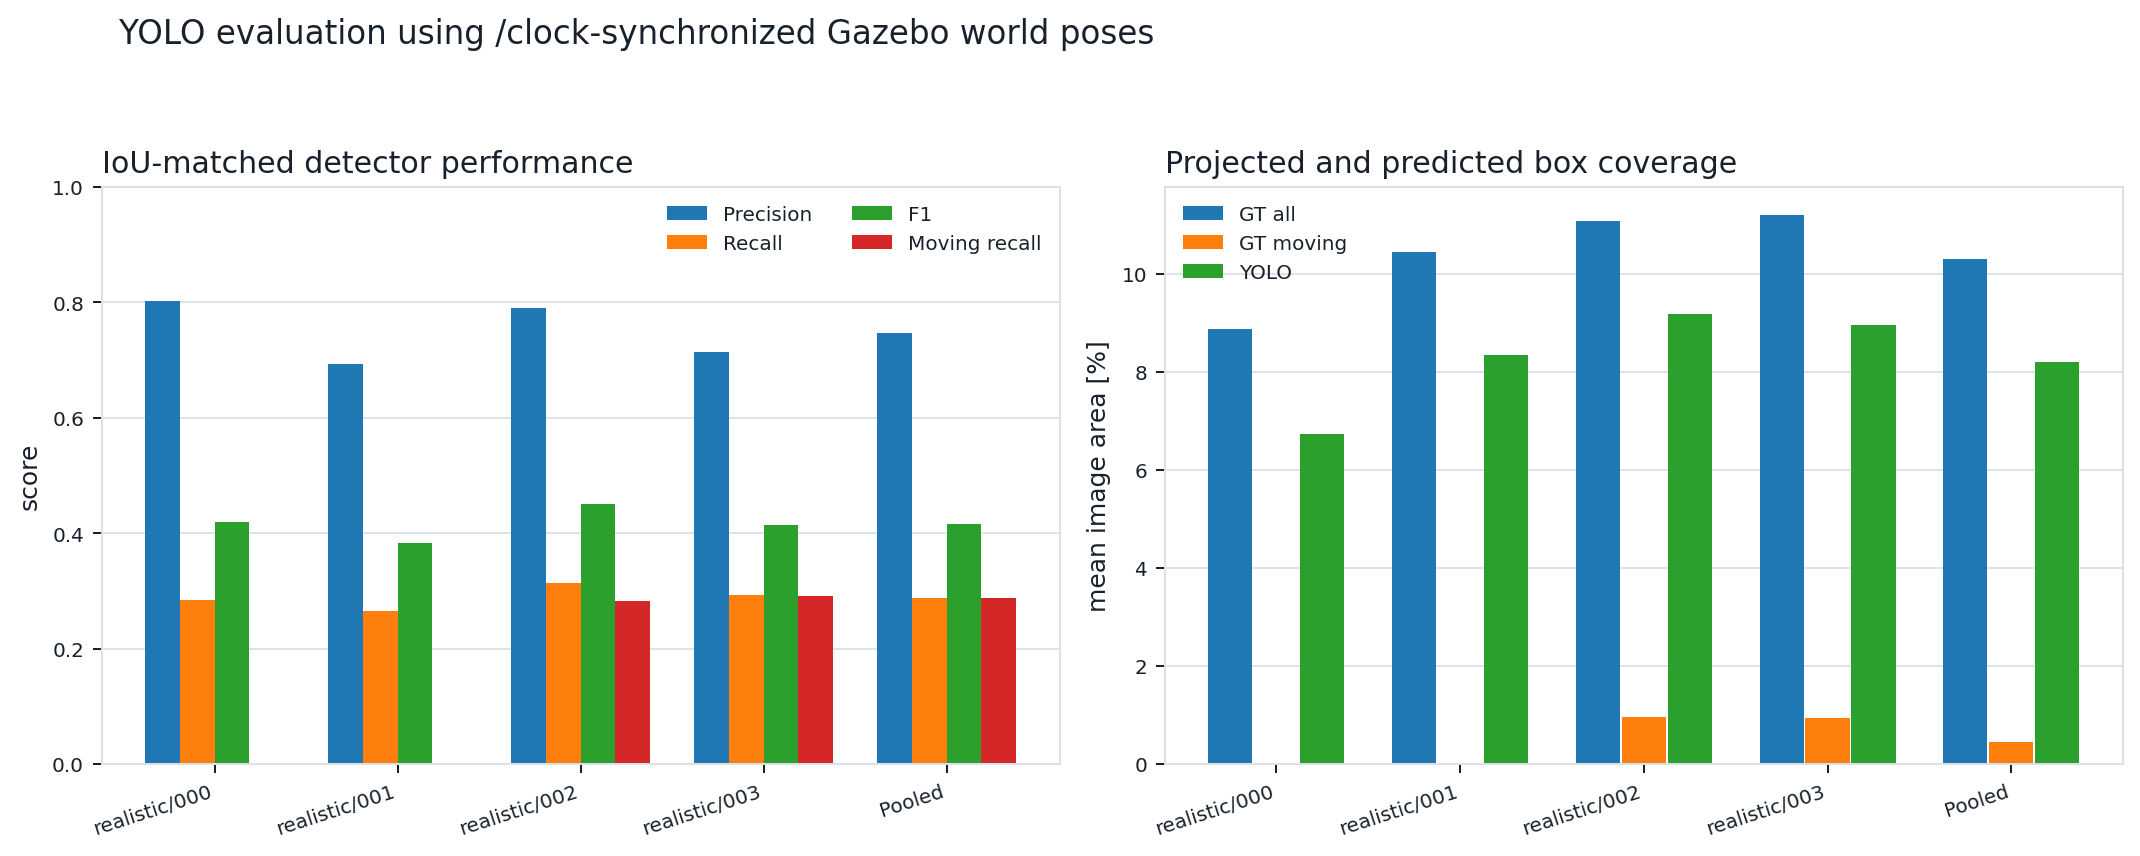
\includegraphics[width=\textwidth]{../../../output/yolo_eval/summary_light.png}
  \caption{Per-recording and pooled detector scores and box-area coverage.
  Pooled values come from pooled counts, not from averaging the four
  recording scores.}
  \label{fig:exp2-summary}
\end{figure}

\begin{figure}[p]
  \centering
  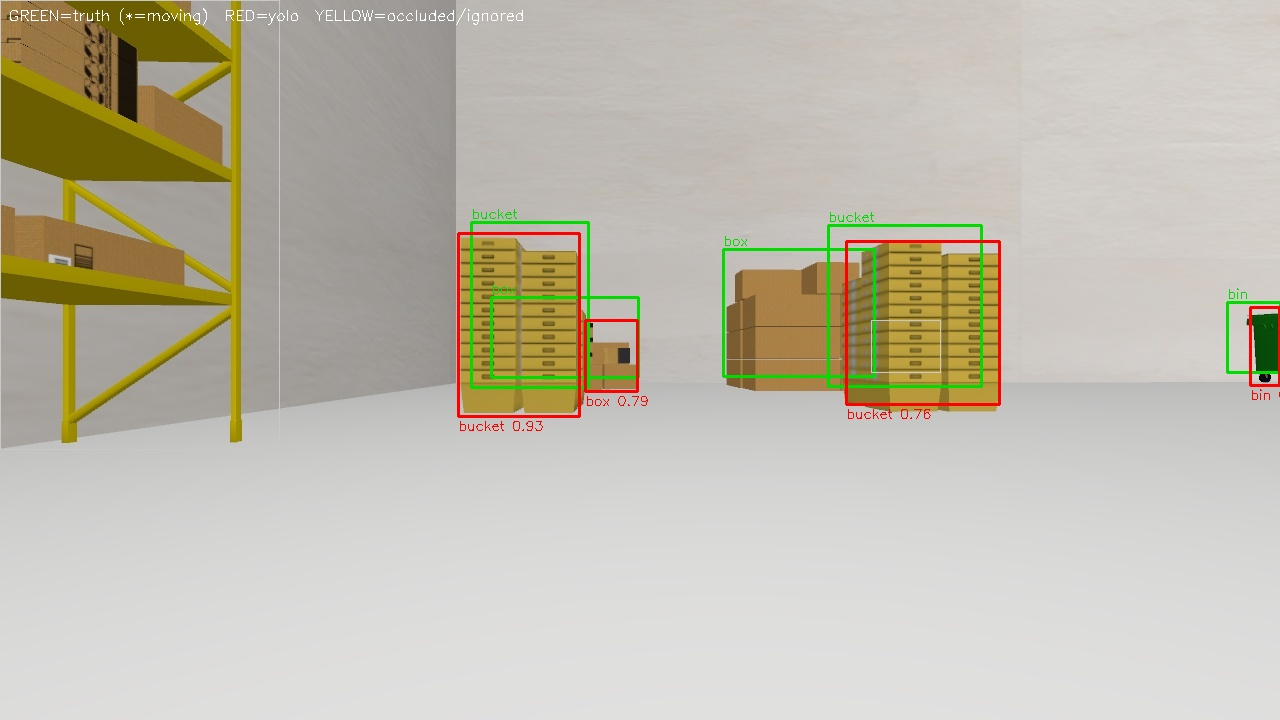
\includegraphics[width=\textwidth]{../../../output/yolo_eval/dyn_00_001/overlay/01116.jpg}
  \caption{Validation overlay of the kind inspected before the metrics were
  accepted (\repo{dynamic_00_001}, frame 01116). Green: projected ground truth,
  scored. Red: predictions. Yellow: truth covered more than \SI{70}{\percent}
  by a nearer object, exempt from scoring. An asterisk marks an object
  classified as moving from its pose history.}
  \label{fig:exp2-overlay}
\end{figure}

\begin{figure}[p]
  \centering
  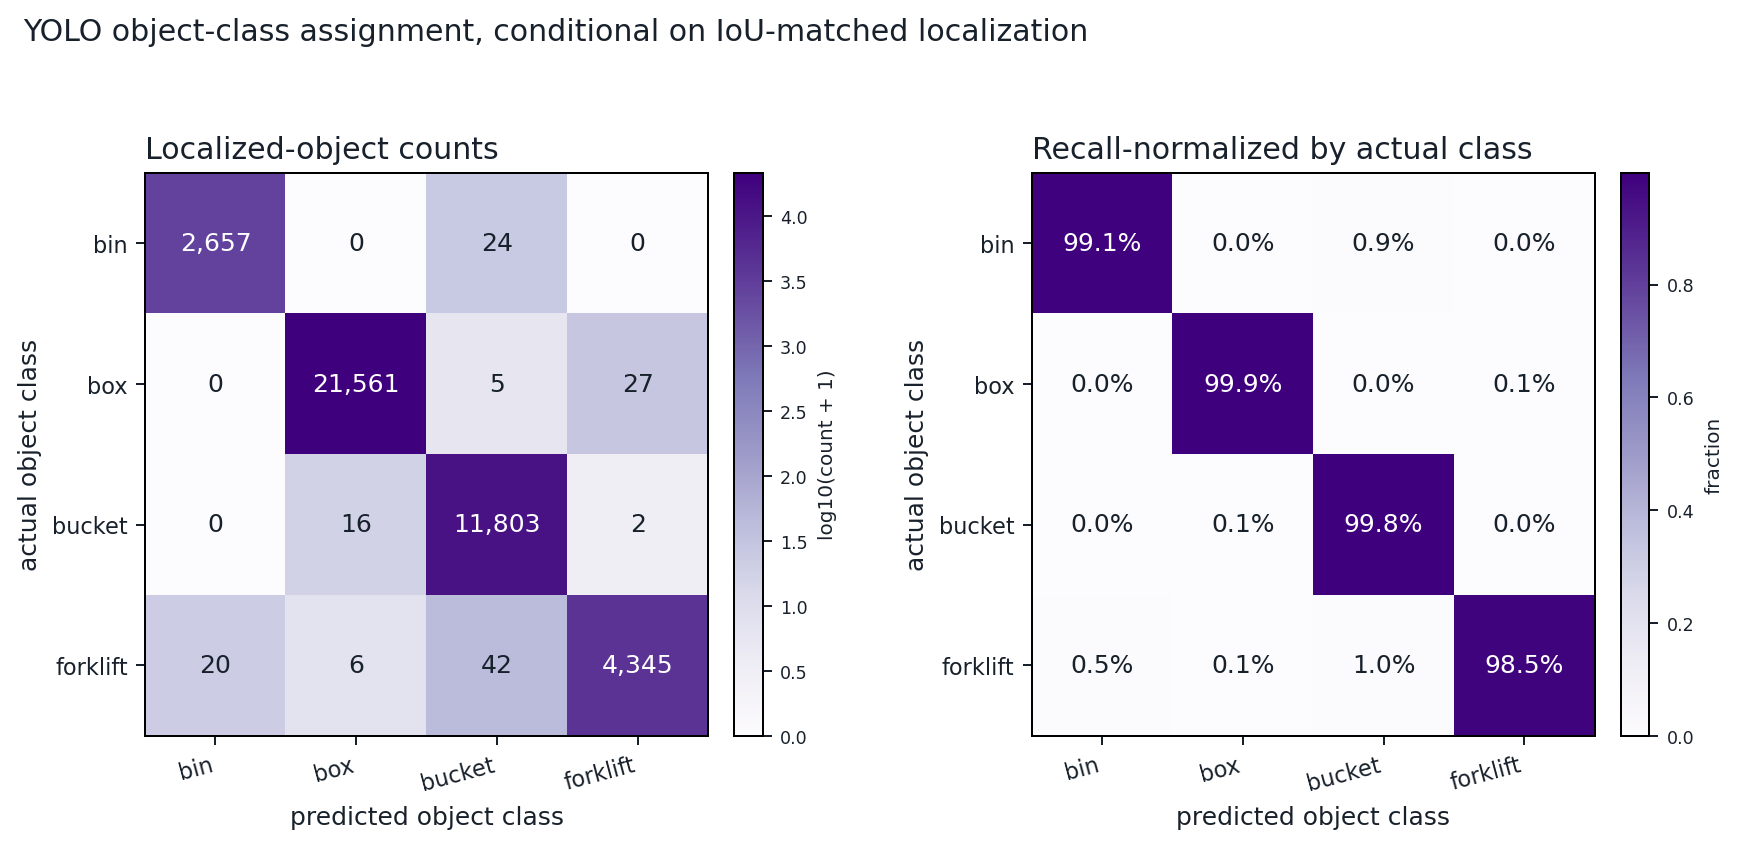
\includegraphics[width=\textwidth]{../../../output/yolo_eval/classification_confusion_light.png}
  \caption{Class confusion conditional on class-agnostic IoU association.
  Rows are true classes, columns predicted. Left: counts on a logarithmic
  colour scale. Right: normalised within each true class. Background is
  excluded by construction.}
  \label{fig:exp2-confusion}
\end{figure}

\paragraph{Analysis.} The recall figure is an upper bound, because it is
computed over the easier subset that the exemptions leave. Of the \num{96758}
projected truth boxes, \num{34476} are exempt as occluded or too small;
counting every one of them as a miss moves pooled recall from \num{0.593} to
\num{0.382}. The training-set validation of the same checkpoint reports
precision \num{0.958} and recall \num{0.882} on human-drawn boxes, so the
drop to \num{0.684} and \num{0.382} on projected boxes mixes a real domain gap
with a stricter scoring convention, and the two cannot be separated without
relabelling a subset by hand.

\emph{Limitation, scoring convention.} Projected boxes are the exact mesh
silhouette, tighter than any annotator draws; a detector fitted to loose human
boxes loses IoU here that represents no error on its part. This is the one
difference from the training convention that no setting of the evaluator can
remove.

\begin{queried}[Ground truth never checked by hand]
The projected ground truth was accepted on visual inspection of sampled
overlays only. No frame has been annotated manually, so the agreement between
projected and human boxes, and therefore the size of the convention effect
above, is unmeasured.
\end{queried}

The miss rate bounds every downstream filter. A class mask built from these
detections can at best remove the \SI{59}{\percent} of moving objects that
are found; the remaining \SI{41}{\percent} stay in the image and reach the
feature extractors of both pipelines regardless of how the mask is applied.
That bound, not the mask mechanism, is the first thing Experiment~3 inherits.

The result does not bear on the online delivery anomaly of Experiment~3. The
detector produces boxes on every recording offline; a filter arm that logged
zero masks failed at message delivery or timestamp matching, which is a
different mechanism from detector capability.

\paragraph{Summary.} The detector names what it finds almost perfectly and
finds about six moving objects in ten, or fewer than four in ten when exempt
objects are counted. Precision \num{0.684} means one prediction in three is a
false box. These are the input limits of the dynamic filters tested in
Experiment~3.

\paragraph{Future plan.} Annotate a stratified subset of frames by hand to
measure the projected-versus-human box convention and separate it from the
domain gap. Re-score on the realistic warehouse recordings, where the moving
objects are pallet jacks on logistics jobs rather than scripted props. Add
object velocity from consecutive detections so that a mask can target moving
objects rather than object classes.

% =====================================================================
\FloatBarrier
\section{Real robot}
\label{sec:exp2-real}

\slotstatus{planned}{Real imagery exists; no real ground-truth boxes do.}

\paragraph{Reason.} Projected ground truth needs object poses and meshes,
which the real site does not provide. The three real recordings hold
\numrange{2562}{3405} usable stereo pairs each, so the detector can be run on
them, but nothing can score it until frames are annotated by hand.

\paragraph{Next action.} Annotate a stratified frame subset of
\repo{dataset_real_000} to \repo{dataset_real_002} across the three
illumination levels of the test site, run the detector at the thresholds of
\cref{sec:exp2-sim}, and report the same metrics. The same annotated subset
calibrates the projected and manual box conventions against each other for the
simulation slot.

\end{document}
